% Slides for talk on hydrogen fuel cells
% given in the department on October 27, 2003.
% 
% The original slides were in Prosper.  This file contains the
% translation of the original slides to Beamer.
% 
% Rouben Rostamian <rostamian@umbc.edu>
% August 31, 2004

\documentclass[10pt]{beamer}
\usetheme{umbc4}
\useinnertheme{umbcboxes}
\setbeamercolor{umbcboxes}{bg=violet!12,fg=black}

\usepackage{rotating} % for defining \schwa
\newcommand{\schwa}{\raisebox{1ex}{\begin{turn}{180}e\end{turn}}}

\newcommand{\arcsinh}{\mathop\mathrm{arcsinh}\nolimits}
\newcommand{\arccosh}{\mathop\mathrm{arccosh}\nolimits}
\newcommand{\Pu}{P_{\mathrm{amb}}}

\title{Hydrogen Fuel Cells}
\subtitle{Modeling and Computations}
\author[R. Rostamian]{Rouben Rostamian}
\institute[UMBC]{
  Department of Mathematics and Statistics \\
  University of Maryland Baltimore County \\
  Baltimore, MD 21250, USA
}
\date{October 27, 2003}
\begin{document}

%----------- titlepage ----------------------------------------------%
\begin{frame}[plain]
  \titlepage
\end{frame}

%----------- slide --------------------------------------------------%
\begin{frame}
  \frametitle{Acknowledgment}

Fred Gornik, Power+Energy, Inc.
\medskip

http://powerandenergy.com

\end{frame}

%----------- slide --------------------------------------------------%
\begin{frame}
  \frametitle{Overview of the talk}

\begin{itemize}
  \item The workings of a hydrogen fuel cell
  \item A mathematical model for hydrogen-palladium interaction
  \item Two mathematical problems:
  \begin{itemize}
    \item Solution and analysis of an ODE
    \item Solution and analysis of a PDE
  \end{itemize}
\end{itemize}

\end{frame}

%----------- slide --------------------------------------------------%
\begin{frame}
  \frametitle{Hydrogen fuel cells: overview}

\begin{center}
  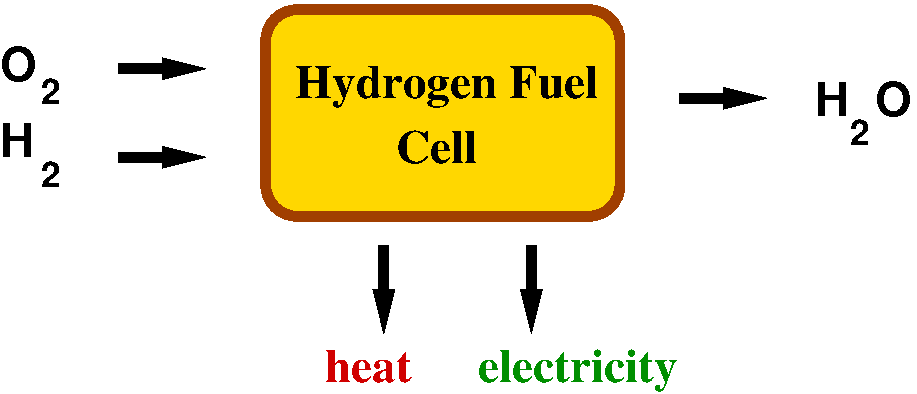
\includegraphics[height=3.0cm]{schematic1.pdf}
\end{center}
\bigskip

\pause

\begin{center}
  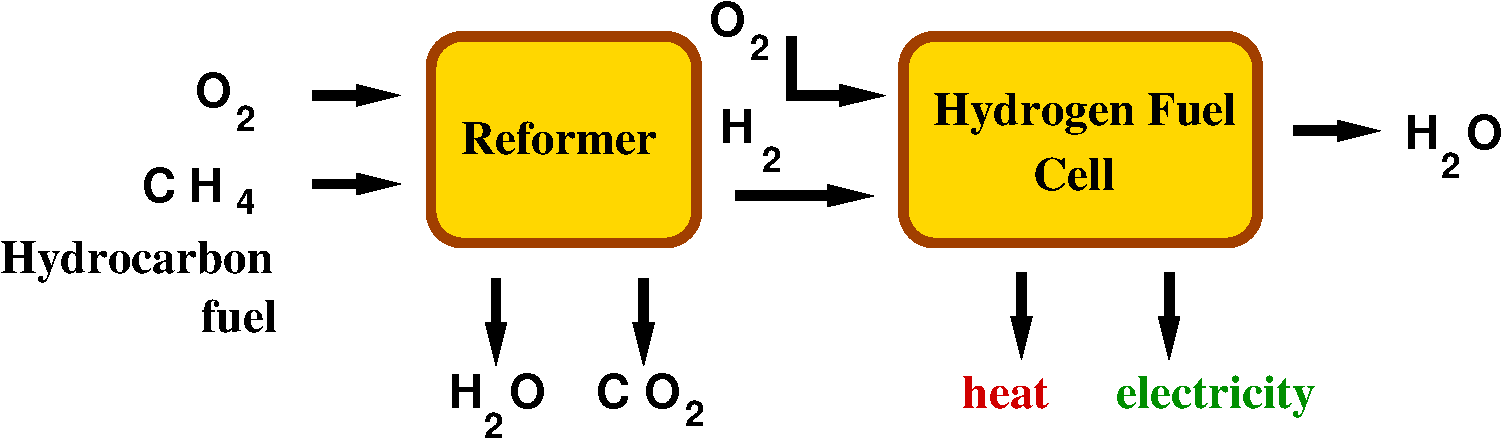
\includegraphics[height=3.0cm]{schematic2.pdf}
\end{center}

\end{frame}

%----------- slide --------------------------------------------------%
\begin{frame}
  \frametitle{Palladium: the element}

\small

\textbf{pal�la�di�um$^{\mathbf{1}}$}
(p\schwa-l$\bar{\textbf{a}}'$d$\bar{\textrm{e}}$-\schwa m) \textbf{n}.\newline
Symbol \textbf{Pd} \newline
1. A soft, ductile, steel-white, tarnish-resistant, metallic element
occurring naturally with platinum, especially in gold, nickel,
and copper ores. Because it can absorb large amounts of hydrogen,
it is used as a purification filter for hydrogen and a catalyst in
hydrogenation.  It is alloyed for use in electric contacts, jewelry,
nonmagnetic watch parts, and surgical instruments.  Atomic number 46;
atomic weight 106.4; melting point 1,552$^\circ$~C; boiling point
3,140$^\circ$~C; specific gravity 12.02 (20$^\circ$~C); valence 2,
3, 4.  See note at \textbf{element}.
\smallskip

[From \textbf{Pallas} (discovered at the same time as the element)]

\bigskip

\pause

\textbf{Pal�las} (p\textbf{\u{a}}l$'$\schwa s) \textbf{n.}\newline
\textbf{1.} One of the largest asteroids, the second to be discovered.\newline
\textbf{2.} \textit{Greek Mythology} Athena.
\smallskip

[After \textbf{Pallas} (Athena)]

\end{frame}

%----------- slide --------------------------------------------------%
\begin{frame}
  \frametitle{The Hydrogen-Palladium interface}

$\Gamma_0 = $ rate of hydrogen molecules impacting a surface

Representative value: $10^{19}$ hits/cm$^2$/sec

$\Gamma_0$ \emph{proportional} to pressure

\bigskip

\begin{columns}
  \begin{column}{.6\textwidth}
    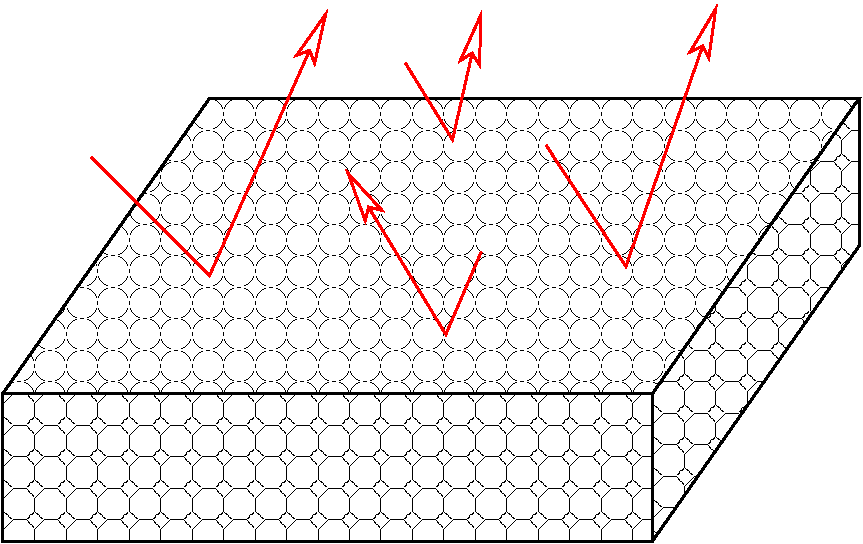
\includegraphics[width=0.8\textwidth]{bounce.pdf}
    \smallskip

    Around $10^{14}$ surface sites/cm$^2$
  \end{column}
\pause
  \begin{column}{.3\textwidth}
    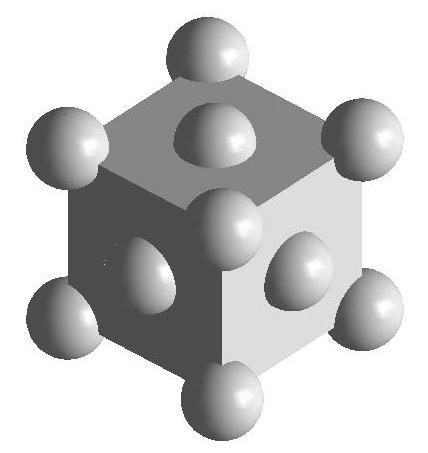
\includegraphics[width=\textwidth]{fcc.jpg}
  \end{column}
\end{columns}

\end{frame}

%----------- slide --------------------------------------------------%
\begin{frame}
  \frametitle{Modeling the surface layer}

Fraction of occupied surface sites on the surface $ = \alpha$, \quad
$0 \le \alpha \le 1$

Rate of sticking $ = \Gamma_0 S_0 (1-\alpha)^2$, \quad $S_0 \approx 0.3$

Rate of recombination $=k_d \alpha^2$

\medskip

\structure{Equilibrium:}
\[
  \Gamma_0 S_0 (1-\alpha)^2 = k_d \alpha^2
  \quad \Rightarrow \quad
  \Bigl(\frac{1-\alpha}{\alpha}\Bigr)^2 = \frac{k_d}{\Gamma_0 S_0}
\]

Fraction of occupied interior sites $ = \beta$, \quad $ 0 \le \beta \le 1$

Flow rate from surface to interior $ = k_i \alpha (1-\beta)$

Flow rate from interior to surface $ = k_o \beta (1-\alpha)$

\medskip

\structure{Equilibrium:}
\[
  k_i \alpha (1-\beta) = k_o \beta (1-\alpha)
  \quad \Rightarrow \quad
  \frac{1-\alpha}{\alpha} = \frac{k_i}{k_o} \frac{1-\beta}{\beta}
\]

\[
  \text{Eliminate $\alpha$:} \qquad
  \frac{\beta}{1-\beta} = \frac{k_i}{k_o}
  \sqrt{\frac{\Gamma_0S_0}{k_d}} 
\]

\end{frame}

%----------- slide --------------------------------------------------%
\begin{frame}
  \frametitle{Diffusion through a membrane}

\[
  \beta \approx 0 
  \quad \Rightarrow \quad
  \beta = C_1 \sqrt{\Gamma_0} = C_2 \sqrt{P}
\]

\medskip

\begin{center}
  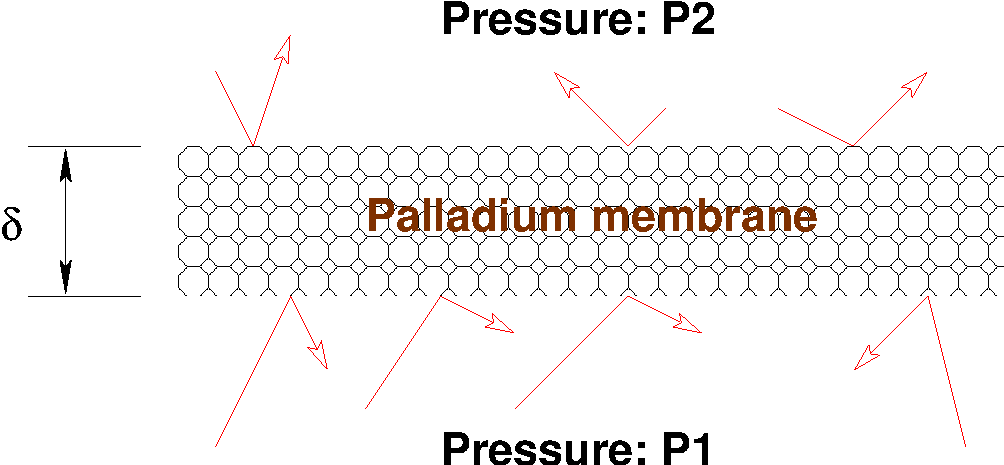
\includegraphics[height=35mm]{p1p2.pdf}
\end{center}

\medskip

Concentrations near the surfaces: $C_2 \sqrt{P_1}$ and $C_2 \sqrt{P_2}$
\[
  \textrm{Flux}
  \: = \: \kappa \:\: \frac{\sqrt{P_1} - \sqrt{P_2}}{\delta}
\]

\end{frame}

%----------- slide --------------------------------------------------%
\begin{frame}
  \frametitle{Flow through a tube}

\begin{center}
  \hspace*{-10mm}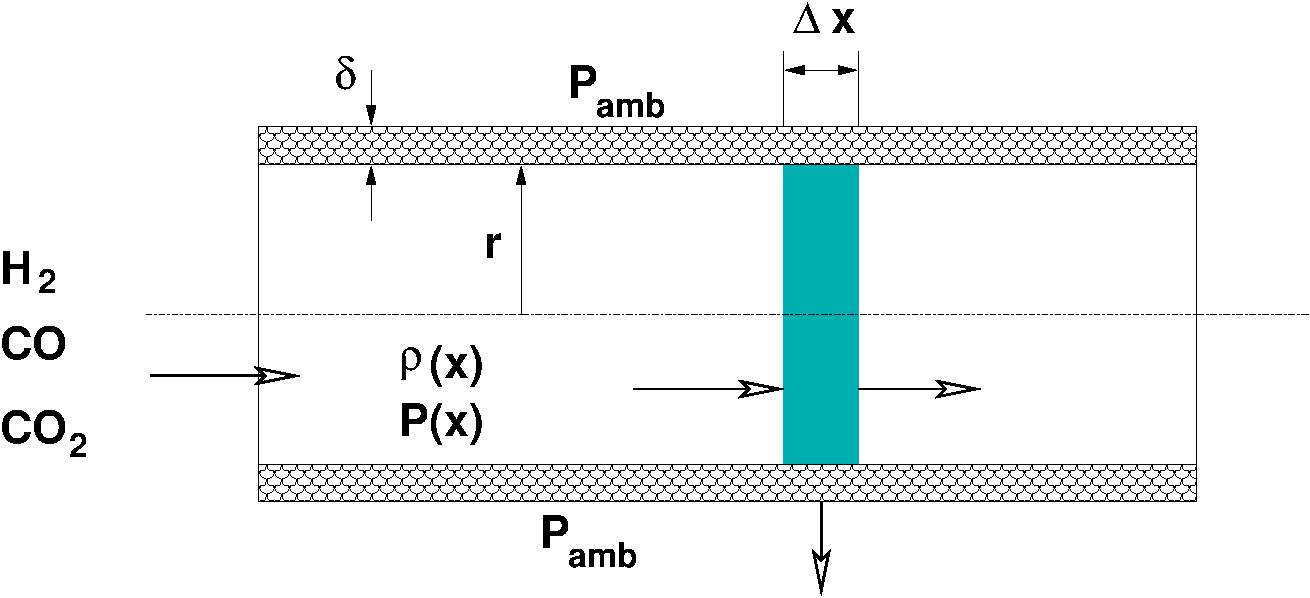
\includegraphics[width=70mm]{tube.pdf} \\
  \textbf{inflow = $\rho A v$} \qquad\qquad
  \textbf{outflow = $(\rho + \Delta \rho) A v$} \\[\medskipamount]
  \textbf{leakage = $\displaystyle(2\pi r \Delta x) \kappa
    \frac{\sqrt{P} - \sqrt{\Pu}}{\delta}$}
\end{center}

\medskip

\structure{Conservation of mass}
\[
  \rho A v = (\rho + \Delta \rho) A v 
    + (2\pi r \Delta x) \kappa \frac{\sqrt{P} - \sqrt{\Pu}}{\delta}
\]

\end{frame}

%----------- slide --------------------------------------------------%
\begin{frame}
  \frametitle{Differential equation of pressure}

\structure{Conservation of mass}
\[
  \frac{d\rho}{dx} = - \frac{2\pi r\kappa}{Av\delta}
  \bigl(\sqrt{P} - \sqrt{\Pu}\:\bigr)
\]

\structure{Ideal Gas}
\[
  P = RT\rho
\]

\[
  \frac{dP}{dx} = - \frac{2\pi r\kappa RT}{Av\delta}
    \bigl(\sqrt{P} - \sqrt{\Pu}\:\bigr)
\]

\structure{Differential equation}
%
\[
  \begin{onlinebox}{5cm}
  $\displaystyle\frac{dP}{dx} = - K \bigl(\sqrt{P} - \sqrt{\Pu}\:\bigr)$,
  \end{onlinebox}
  \qquad
  K = \frac{2\pi r\kappa RT}{F\delta}, \quad F = Av
\]

\end{frame}

%----------- slide --------------------------------------------------%
\begin{frame}
  \frametitle{Calculation of pressure}

\begin{displaybox}{60mm}
\[
  \frac{dP}{dx} = - K \bigl(\sqrt{P} - \sqrt{\Pu}\:\bigr)
\]
\end{displaybox}

\bigskip

\pause

\begin{center}
  Solve for $P(x)$:\qquad
  \begin{onlinebox}{45mm} $\displaystyle P(x) = \Pu [ 1 + W(z)]^2$
  \end{onlinebox}
\end{center}

\bigskip

\[
\text{where } z = \frac
  {\sqrt{P(0)} - \sqrt{\Pu}}{\sqrt{\Pu}}
  \exp\Bigl(\frac{\sqrt{P(0)} - \sqrt{\Pu} - \frac12 Kx}{\sqrt{\Pu}}\Bigr)
\]


\begin{columns}
  \begin{column}{0.4\textwidth}
    $W$: the \textit{Lambert function}
    \bigskip

    $\displaystyle ye^y = x \quad \Leftrightarrow \quad y = W(x)$
  \end{column}
  \begin{column}{0.4\textwidth}
    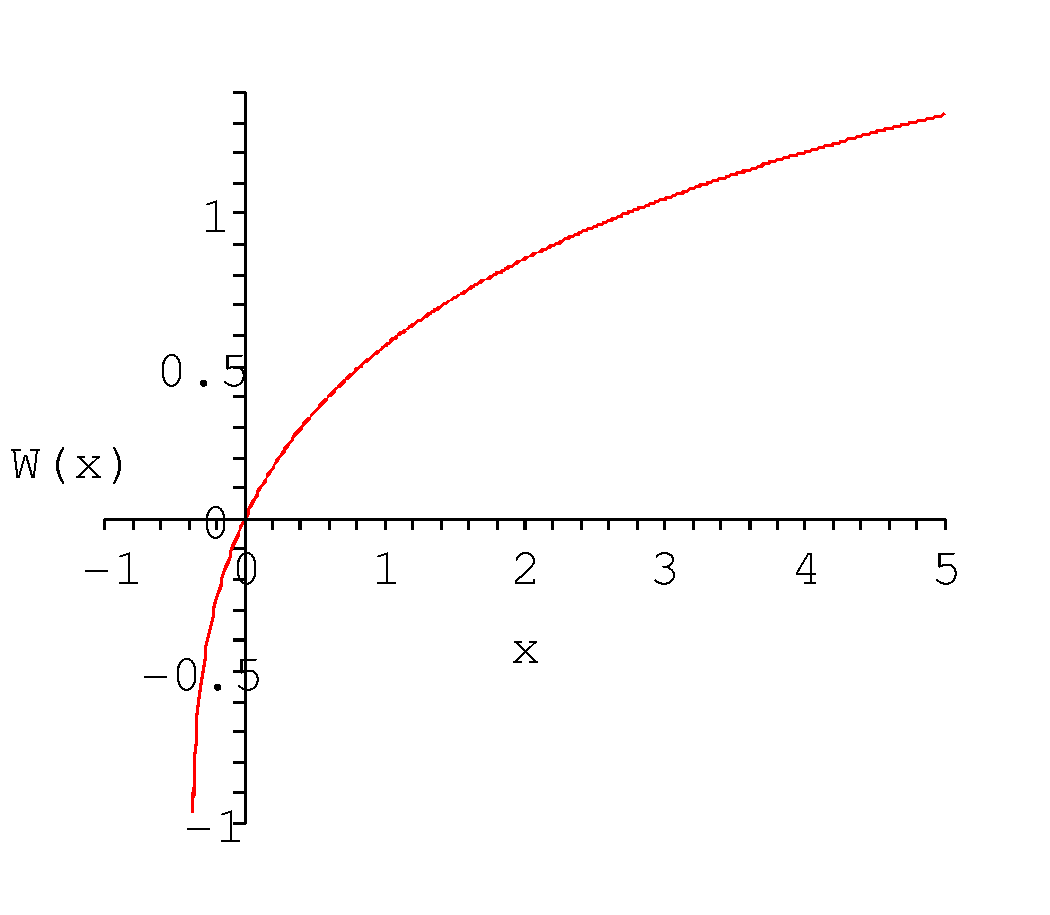
\includegraphics[width=\textwidth]{lambertW.pdf}
  \end{column}
\end{columns}

\end{frame}

%----------- slide --------------------------------------------------%
\begin{frame}
  \frametitle{Efficiency of hydrogen exchange}

Rate of hydrogen inflow = $F\rho(0)$
\medskip

Rate hydrogen outflow = $F\rho(L)$
\medskip

Rate of hydrogen release: $F\rho(0) - F\rho(L)$

\bigskip
\bigskip

\structure{Efficiency:}
\[
\mathcal{E}
  = \frac
    {\text{rate of hydrogen release}}
    {\text{rate of hydrogen inflow}}
  = \frac{F\rho(0) - F\rho(L)}{F\rho(0)}
  = 1 - \frac{\rho(L)}{\rho(0)}
  = 1 - \frac{P(L)}{P(0)}
\]
\bigskip

\structure{Best possible efficiency:}
\[
  \mathcal{E}_{\max} = 1 - \frac{\Pu}{P(0)}
\]

\end{frame}

%----------- slide --------------------------------------------------%
\begin{frame}
  \frametitle{Numbers}

\renewcommand{\arraystretch}{1.7}
\begin{tabular}{lll}
  tube radius & $r$ & 0.3175 cm \\
  tube wall thickness & $\delta$ & 0.0003 cm \\
  flow rate & $F$ & 8330 cm$^3$/sec \\
  inlet pressure & $P(0)$ & 4.08 atm \\
  ambient pressure & $\Pu$ & 1.36 atm \\
  temperature & $T$ & 673 Kelvin \\
  diffusivity & $\kappa$ & 6.96 10$^{-8}$ mol/(cm sec atm$^{1/2}$) \\
  gas constant & $R$ & cm$^3$ atm / (mol Kelvin)
\end{tabular}

\end{frame}

%----------- slide --------------------------------------------------%
\begin{frame}
  \frametitle{Results}

\centerline{
  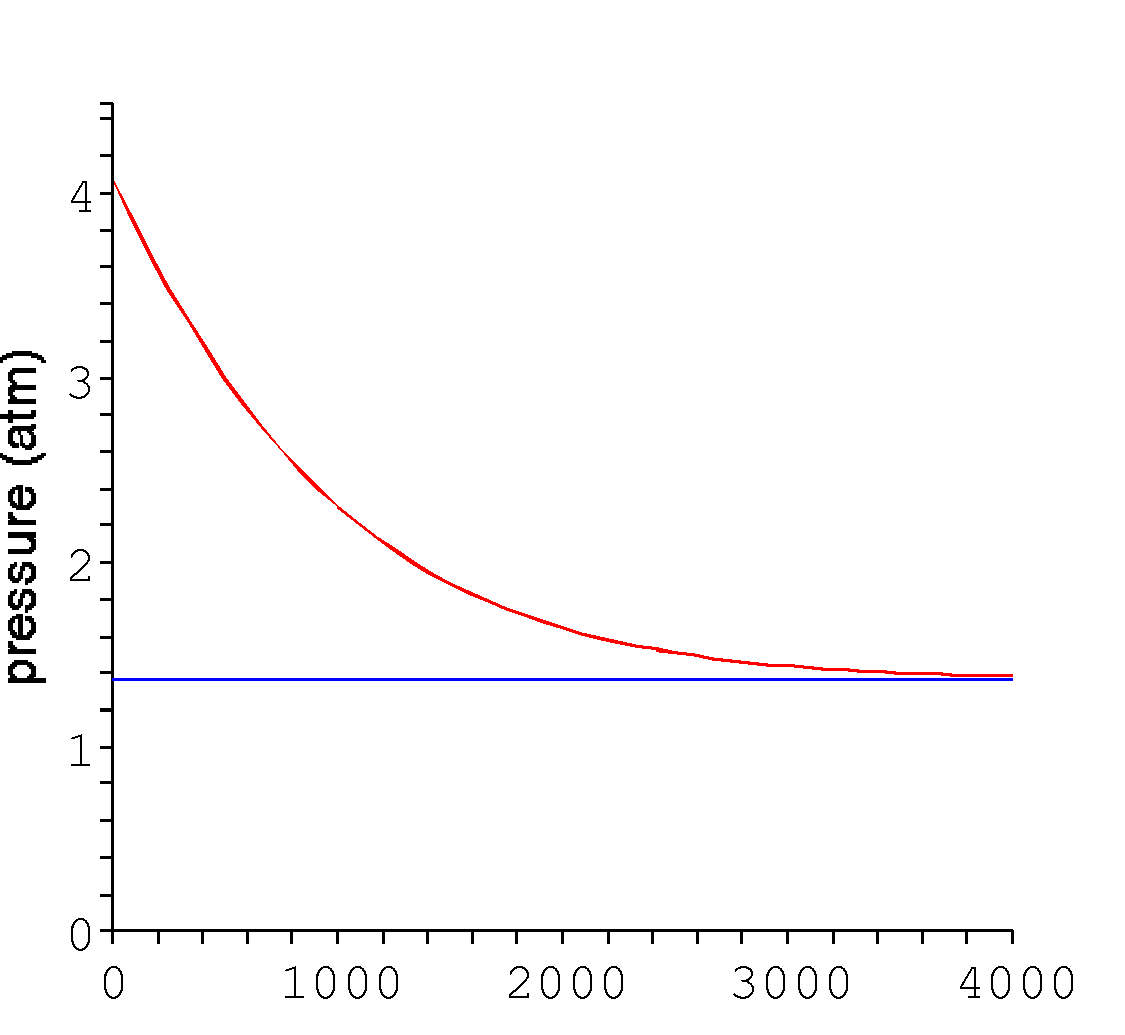
\includegraphics[width=0.4\textwidth]{pressure.pdf}
  \qquad
  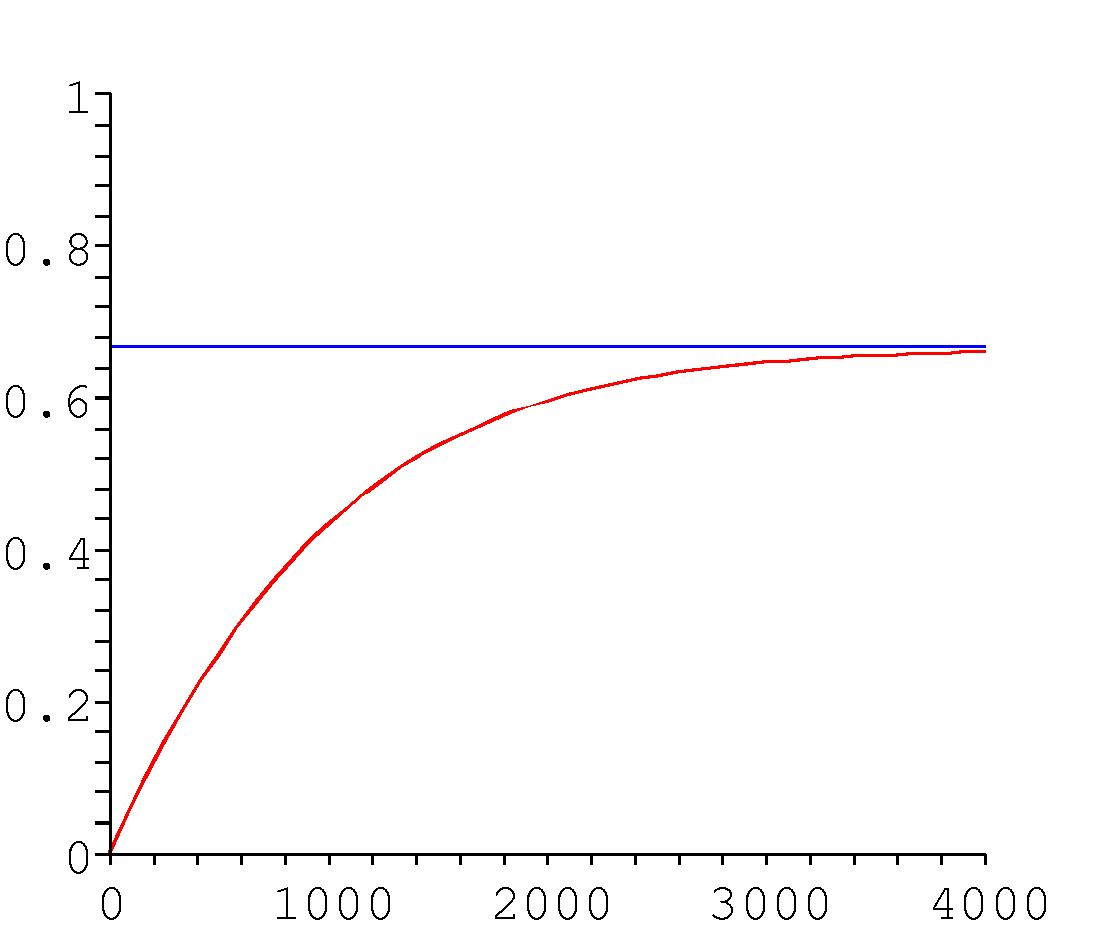
\includegraphics[width=0.4\textwidth]{efficiency.pdf}
}

\end{frame}

%----------- slide --------------------------------------------------%
\begin{frame}[t]
  \frametitle{Membrane on porous support}

\only<1>{
  \centerline{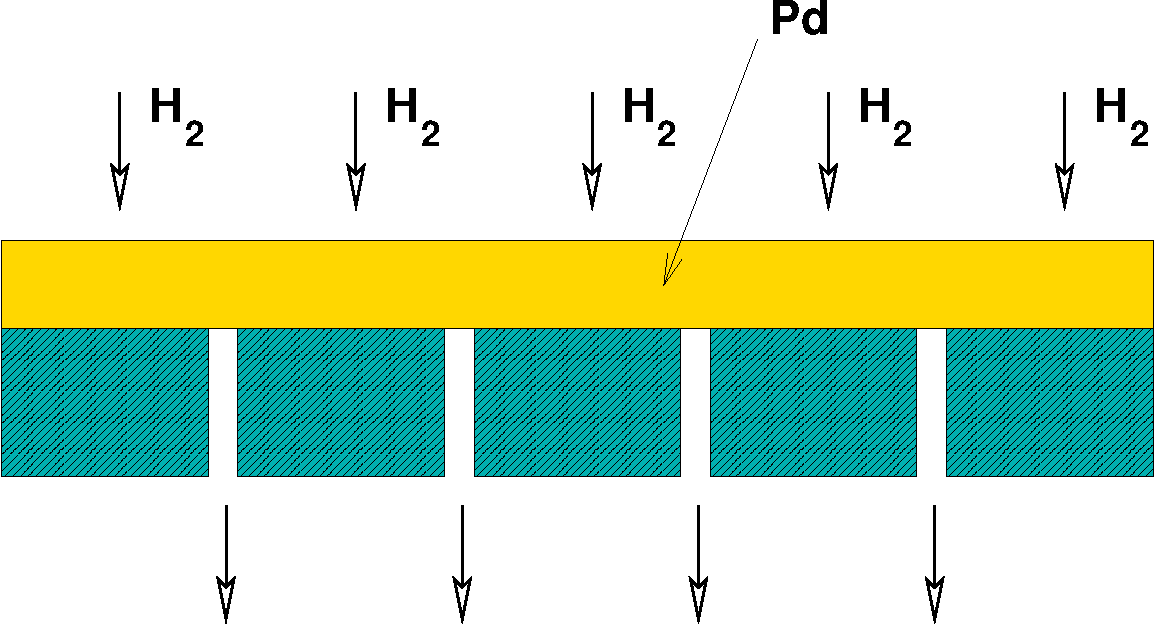
\includegraphics[height=4cm]{bedsupport1.pdf}}
}

\onslide<2->{
  \centerline{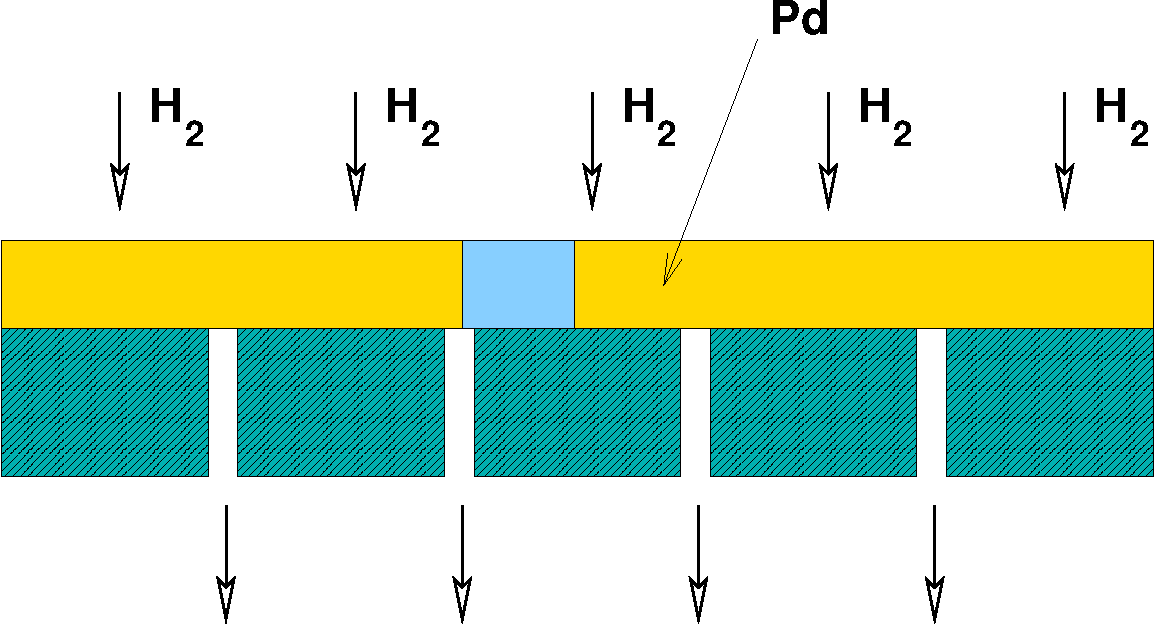
\includegraphics[height=4cm]{bedsupport2.pdf}}
}

\onslide<3->{
\begin{columns}[T]
  \begin{column}{0.3\textwidth}
    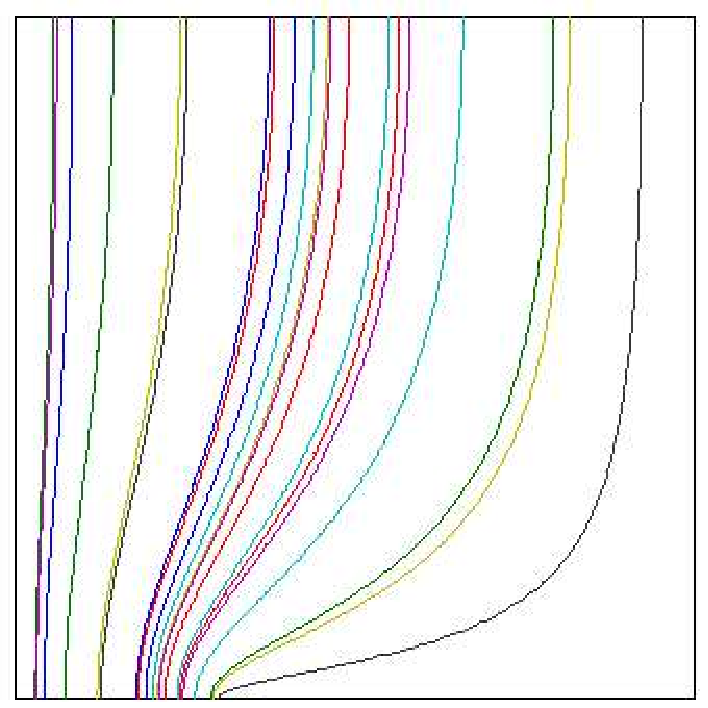
\includegraphics[height=26mm]{cell-lines.pdf}
  \end{column}
  \begin{column}{0.3\textwidth}
    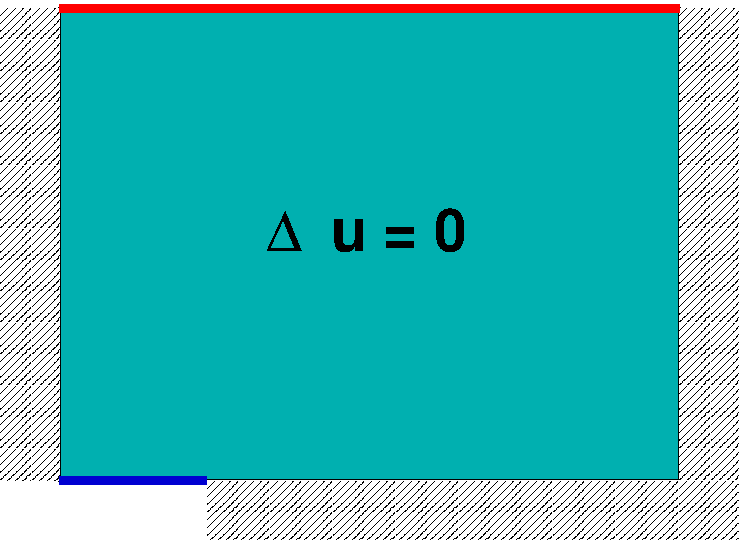
\includegraphics[height=29mm]{bedsupport3.pdf}
  \end{column}
\end{columns}
}

\end{frame}

%----------- slide --------------------------------------------------%
\begin{frame}
  \frametitle{Numerical solution with Femlab}

\begin{center}
  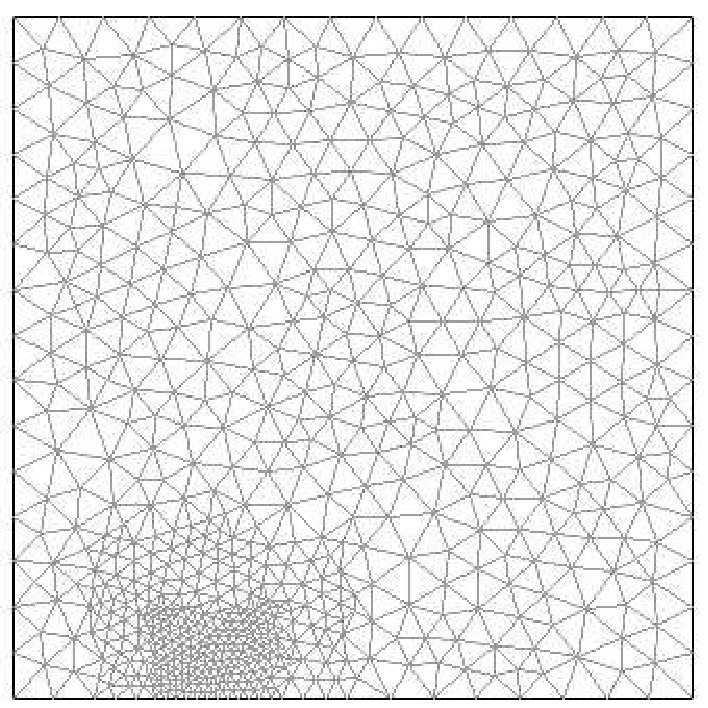
\includegraphics[height=25mm]{cell-mesh.pdf} \qquad\qquad
  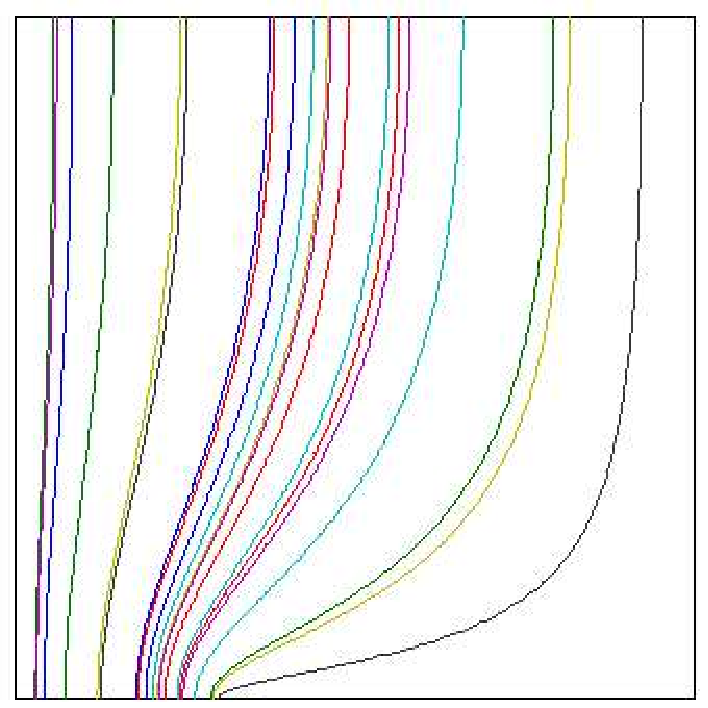
\includegraphics[height=25mm]{cell-lines.pdf} \\[\bigskipamount]
  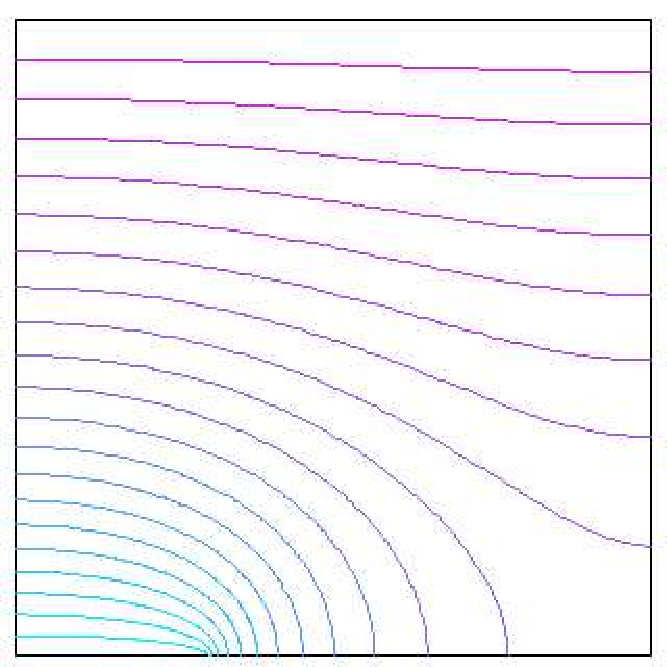
\includegraphics[height=25mm]{cell-contours.pdf} \qquad\qquad
  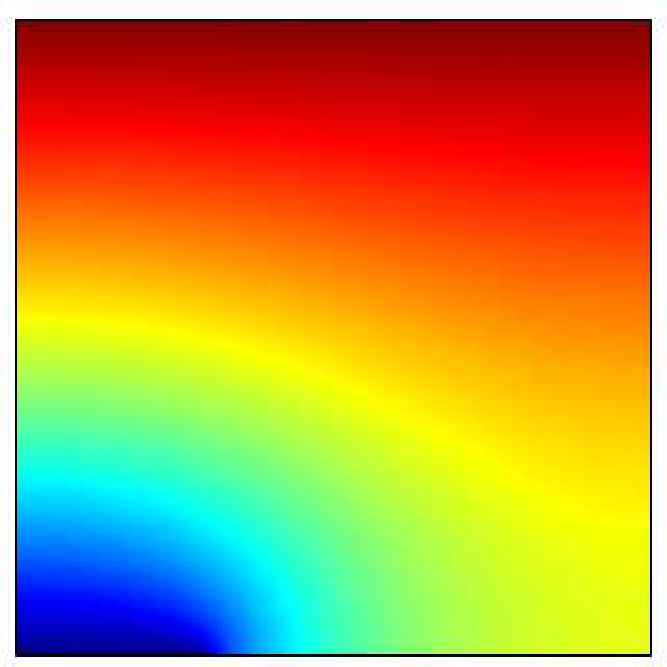
\includegraphics[height=25mm]{cell-shaded.pdf}
\end{center}

\pause

\[
  \int_0^1 \frac{\partial T}{\partial y} (x, 1) \, dx = 0.667
  \qquad
  \int_0^{0.3} \frac{\partial T}{\partial y} (x, 0) \, dx = 0.627
\]

\end{frame}

%----------- slide --------------------------------------------------%
\begin{frame}
  \frametitle{The limiting case}

\begin{columns}
  \begin{column}{0.5\textwidth}
  \[
    \text{Throughput} = J(a)
    = \int_0^a \frac{\partial T}{\partial v}\Big|_{v=0} \, du
  \]
  \end{column}
  \begin{column}{0.4\textwidth}
    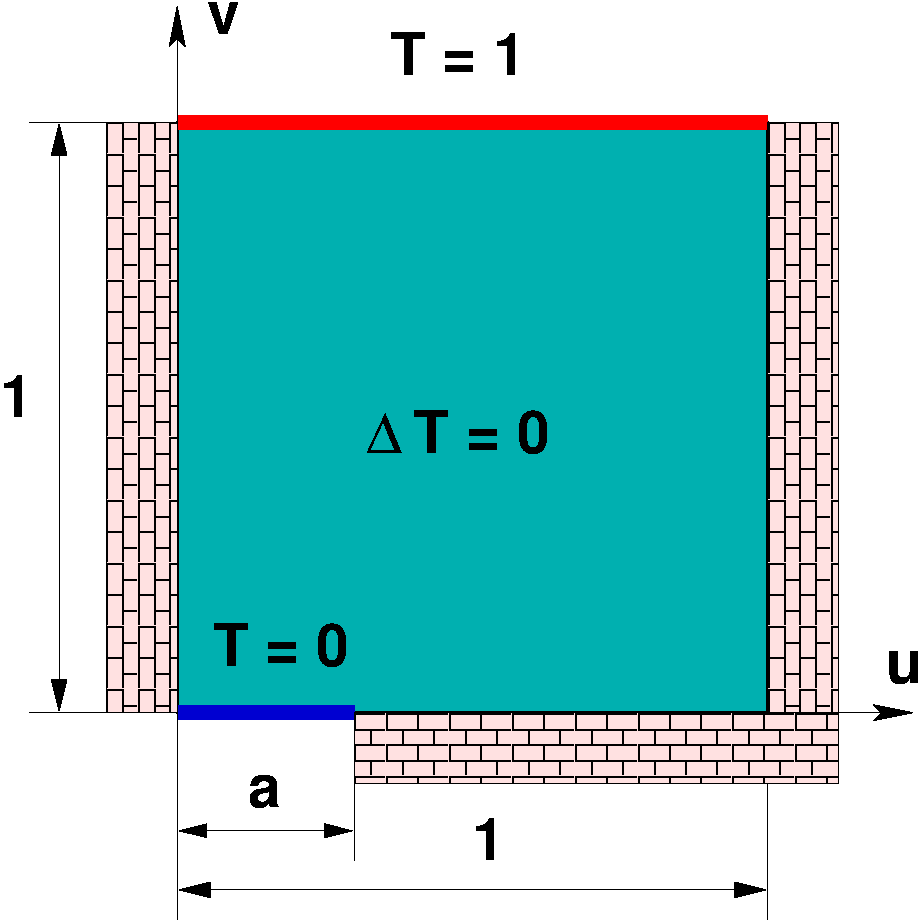
\includegraphics[width=\textwidth]{pde1.pdf}
  \end{column}
\end{columns}

\pause

\begin{theorem}
Asymptotically, as $a\to0$:
\[
  J(a) \approx \frac{\pi}{2\ln \frac2a}.
\]
\end{theorem}

\end{frame}

%----------- slide --------------------------------------------------%
\begin{frame}
  \frametitle{Conformal mapping}

\begin{center}
  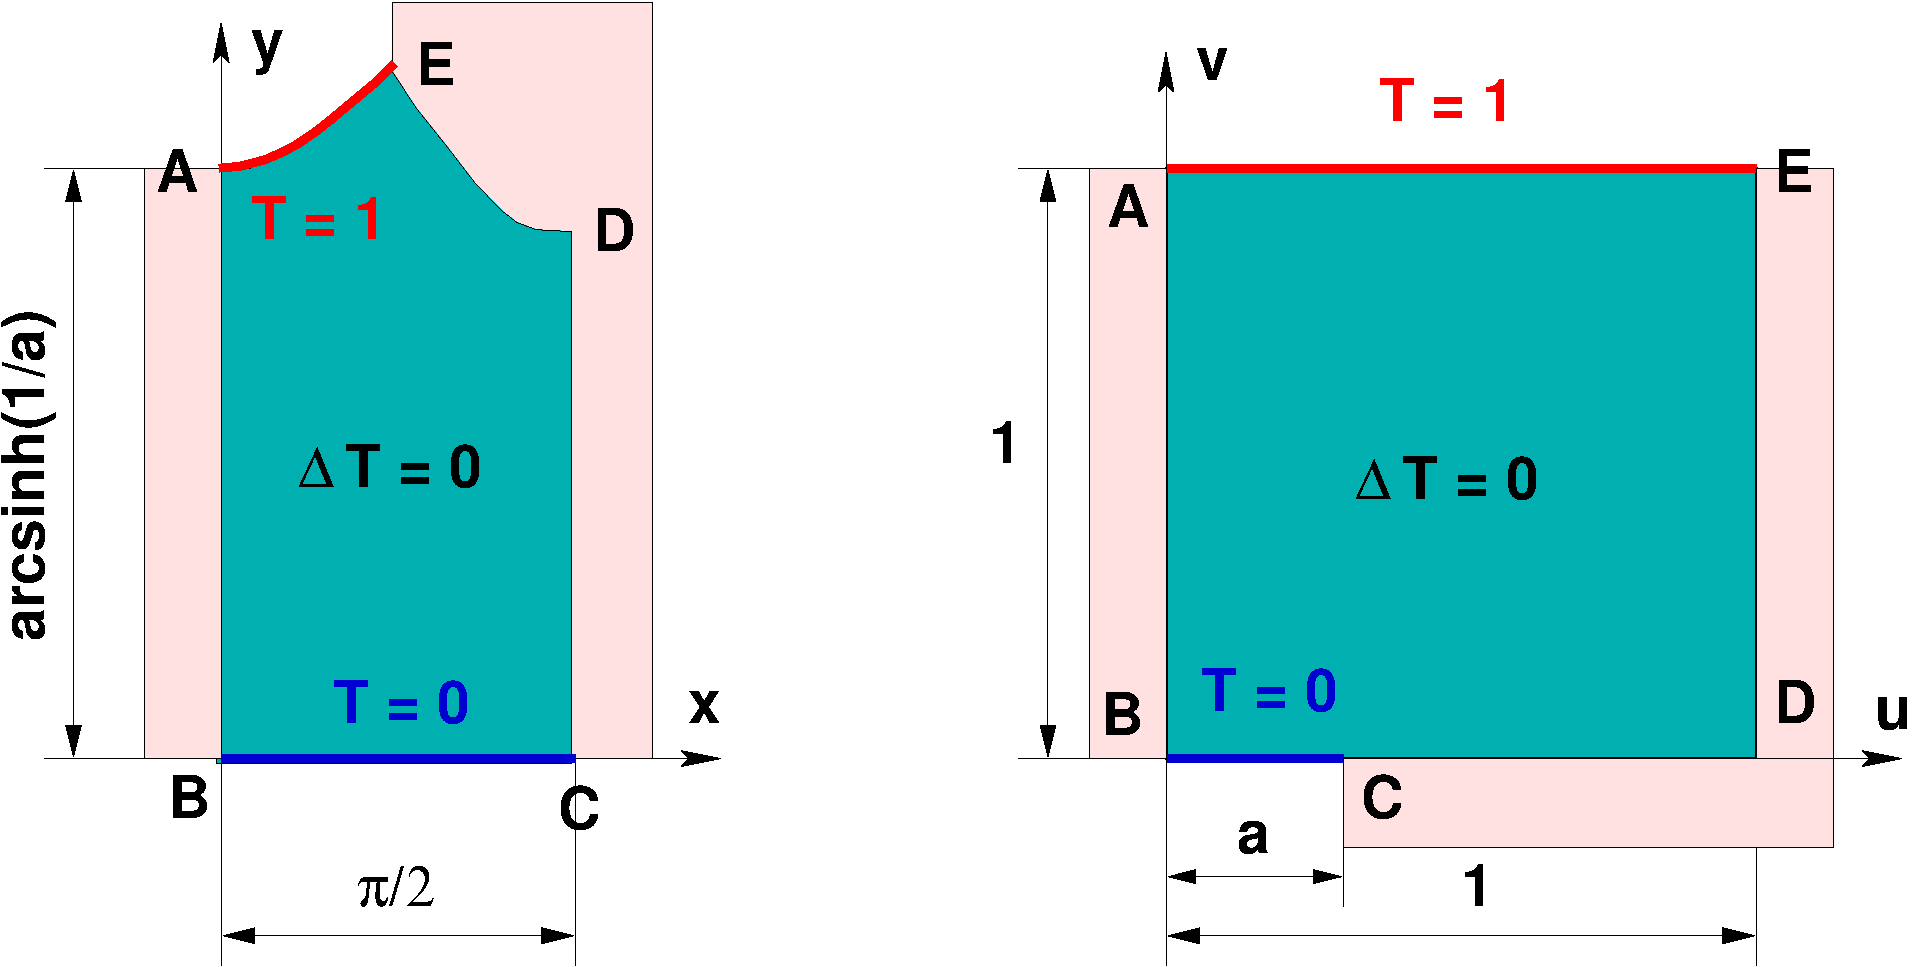
\includegraphics[height=42mm]{pde2.pdf}
\end{center}

\begin{gather*}
  u + iv = a \sin(x + iy) 
  \quad \Leftrightarrow \quad
  u = a \sin x \cosh y,  \quad v = a \cos x \sinh y
\end{gather*}

\pause 

\[
  T = T(x,y) \approx \frac{y}{\arcsinh(1/a)}
\]

\end{frame}

%----------- slide --------------------------------------------------%
\begin{frame}[t]
  \frametitle{Proof of theorem}

\small
\[
  T(u,v) \approx  
  \frac{1}{\arcsinh\frac1a} \arccosh \left[ \frac{1}{2} 
    \sqrt{\Bigl(\frac{u}{a}+1\Bigr)^2 + \Bigl(\frac{v}{a}\Bigr)^2}
    + \frac{1}{2} \sqrt{\Bigl(\frac{u}{a}-1\Bigr)^2 +
    \Bigl(\frac{v}{a}\Bigr)^2} \right]
\]
\normalsize

\bigskip
\pause

\[
  J(a) = \int_0^a \left. \frac{\partial T(u,v)}{\partial v} \right|_{v=0}
    \,du = ?
\]  

\pause

\[
  \left.\frac{\partial T(u,v)}{\partial v}\right|_{v=0} = 
    \frac{1}{a\arcsinh\frac1a} \frac{1}{\sqrt{1-(\frac{u}{a})^2}}
    \qquad\qquad \text{(calculus challenge!)}
\]

\bigskip
\pause

\[
  J(a) = \int_0^a \left. \frac{\partial T(u,v)}{\partial v} \right|_{v=0}
    \,du
    =
    \frac{\pi}{2\arcsinh\frac1a}
    \approx
    \frac{\pi}{2\ln \frac2a} \qquad QED
\]

\end{frame}

\end{document}
